\capitulo{3}{Conceptos teóricos}

Algunos conceptos teóricos tanto de la parte técnica como de la parte de procesos de software


\section{Deuda técnica}

La metáfora de deuda nació cómo una forma de expresar la diferencia entre el entendimiento del programa (la abstracción) y su implementación \cite{cu09}.

Con el tiempo nació un termino similar la deuda técnica que es la metáfora que expresa el coste que conlleva el dejar código que no tiene un buen diseño en el proyecto. Si seguimos manteniendo el proyecto esta deuda cada vez costará más el arreglarla y tendremos que pagar los intereses \cite{fow03}.

Las razones de incremento de la deuda con el paso del tiempo pueden ser el simple hecho de olvidar como funciona cada linea de código, o la complejidad emergente del acoplamiento de código antiguo con otro nuevo sin cambiar las abstracciones ni desacoplar el código.

\begin{figure}
	\centering
	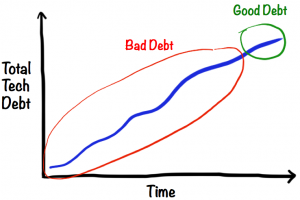
\includegraphics[width=0.8\textwidth]{deuda1.png}
	\caption{Deuda técnica: Beneficiosa y perjudicial.\cite{kni13}}\label{fig:deuda1.png}
\end{figure}


Este tipo de deuda se ve como necesaria, según algunos autores \cite{kni13} se debe incurrir en deuda técnica ya que es beneficioso para el desarrollo. Esto se debe a que a corto plazo es imposible prever cómo se va a desarrollar el proyecto y unos cambios demasiado tempranos pueden ser un mal diseño a medio o largo plazo. La deuda `buena' o beneficiosa se suele considerar como aquella que como mucho dura una semana, una vez existe por más tiempo pasa a ser cada vez más costosa de solucionar o `pagar'.


Una característica importante de esta deuda es que una vez dejas de soportar el mantenimiento de un proyecto la deuda técnica desaparece, al contrario que la deuda financiera.

Se puede idealizar la deuda técnica y considerar que todas las semanas en las que se dedica una cantidad de tiempo a solucionarla esta deuda técnica desaparece, pero esto no corresponde con la realidad. Normalmente la deuda aunque se solucione suele ir incrementando poco a poco debido a la complejidad de un sistema mantenido a lo largo de una gran cantidad de tiempo.

La manera de tener esto en cuenta es tener un `techo de deuda' este techo debería ser lo suficientemente alto como para que no se alcance todos los meses pero no demasiado alto como para que cuando se llegue el proyecto sea directamente un fracaso o demasiado caro de pagar.

La opinión de algunas personas parece ser que se debe llegar al techo cada 6 meses, desde mi propia inexperiencia creo que deberíamos evaluar la deuda a los 4 meses para ver si la re-estructuración del proyecto es viable e intentar buscar un punto de tiempo en el que el pagar la deuda técnica sea algo más simple ya que si esperamos hasta los 6 meses probablemente no podamos elegir un momento óptimo. 

\begin{figure}
	\centering
	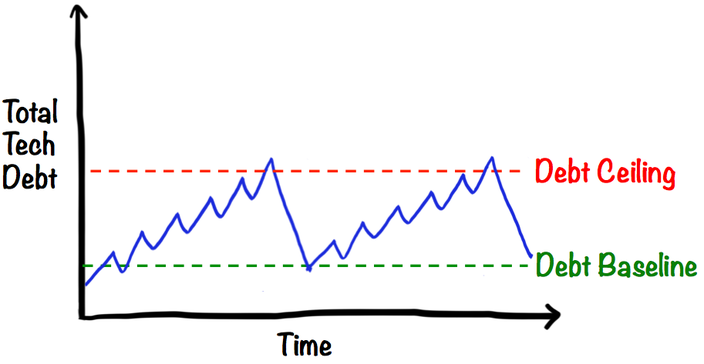
\includegraphics[width=0.8\textwidth]{deuda2.png}
	\caption{Deuda técnica: Techo y base \cite{kni13}}\label{fig:deuda2.png}
\end{figure}

Es importante destacar que la deuda técnica tiene otros razonamientos para tener que mantenerse baja: al que menos importancia parece darse es que la deuda técnica es algo difícilmente cuantificable hasta que se refactoriza, si no la reducimos no sabemos cuanta tenemos.

\section{Integración continua (\textit{Continuous Integration})}

Normalmente acortado con las siglas CI, es un método habitual para reducir la deuda técnica. Es la práctica de ejecutar y testear conjuntamente todas los servicios que deban ir relacionados una vez se inicie el despliegue en producción. Esto nos asegura que van a funcionar en producción la mayoría de las veces, la minoría habrá problemas por la escalabilidad, errores dado el cambio del hardware, problemas con el rendimiento\ldots Un ejemplo es si ejecutamos java y los test no fallan pero al ponerlo en producción le damos a la JVM más de 200 GB de memoria RAM, esto causa comportamientos inesperados.

\subsection{Entrega continua (Continuous Delivery)}

Es un término asociado a CI, consiste en un proyecto que dispone de CI y buena cantidad de test de calidad, una vez ya tengamos un sistema a punto podemos empezar a modificar o mejorar funcionalidades añadiéndolas directamente a producción si pasa los test, requiere que hagamos los test casi a la vez que el código. Esto fomenta y premia técnicas como extreme programming (XP) que se basan en TDD (Test Driven Development), una forma de programar que pide que hagamos los test antes que el resto del código.


\section{DevOps}

DevOps es un acrónimo inglés de: `software \textbf{Dev}elopment and information technology \textbf{Op}eration\textbf{s}' es un termino que engloba un conjunto de prácticas de colaboración y comunicación entre desarrolladores software y técnicos informáticos. Los objetivos de esta comunicación y colaboración son una construcción de software más consistente y confiable. Este proceso heredero de las técnicas ágiles se basa en una \textit{cadena de herramientas}. Esta cadena de herramientas es algo que no esta completamente definida pero más o menos la podemos concretar, cabe tener en cuenta que esta cadena cambia según a quien le preguntes.

\subsection{La `cadena de herramientas' de DevOps}

Esta cadena de herramientas se basa en siete procesos con sus correspondientes herramientas:

\begin{enumerate}
 \item Plan: Consistente en determinación de métricas, requerimientos\ldots y una vez pasemos de la primera iteración ha de tener en cuenta el feedback del cliente.
 \item Creación: Es el proceso de programar y crear el software, las herramientas en este proceso es el software de control de versiones que vayamos a usar.
 \item Verificación: Proceso de comprobación de la calidad del software. Normalmente consiste en hacer test de diversos tipos (Aceptación, seguridad\ldots)
 \item Preproducción o empaquetación: En esta fase se piden aprobaciones de los distintos equipos y se configura el paquete.
 \item Lanzamiento: En este punto se prepara el horario de lanzamiento y se orquesta el software para poder ponerlo en el entorno de producción objetivo.
 \item Configuración: Una vez el software esta desplegado toda la parte de la infraestructura y configuración de la misma se incluye en esta categoría, como por ejemplo las bases de datos, configuración de las mismas\ldots 
 \item Monitorización: Tras entregar el software se mide su rendimiento en la infraestructura objetivo y se mide la satisfacción del usuario final. Se recogen métricas y estadísticas
\end{enumerate}


\section{Microservicios}

Los microservicios son una arquitectura y un patrón de diseño, que no se ha inventado en un momento dado, si no que ha surgido como una tendencia o patrón del diseño de sistemas en el mundo real. 

Un microservicio es un servicio pequeño y autónomo que puede trabajar junto a otros, es importante que este centrado en hacer una cosa bien.

Esto esta reforzado por el concepto del Principio de responsabilidad única de C. Martin\cite{martin03} "Juntar aquellas cosas que cambian por la misma razón y separar aquellas que cambian por razones diferentes."

El tamaño de un microservicio es algo muy discutido, pero generalmente se requiere que sea mantenible por un equipo 'pequeño' (6-10 personas), y se pueda reescribir en 2 semanas.

Esto se debe conseguir mediante una interfaz de programación de aplicación (API: application programming interface), que permita a los clientes acceder al servicio sin causar acoplamiento, algo más difícil de hacer que de decir.

Los principales beneficios son:
\begin{enumerate}
\item Sistemas heterogéneos: Facilita usar distintas tecnologías en distintos sistemas para usar la mejor herramienta en cada ocasión.
\item Resiliencia: Si falla un microservicio el resto del sistema se puede mantener levantado, aislando los problemas y facilitando la alta disponibilidad.
\item Escalabilidad: En caso de que una parte del sistema necesite mayor número de recursos podemos crear una nueva instancia sin cambiar el funcionamiento del resto del sistema.
\item Facilidad de despliegue: Los cambios se mantienen más contenidos.
\item Replazabilidad: Un microservicio que pasa a ser obsoleto puede ser reemplazado o eliminado en vez de tener que mantenerlo por que al eliminarlo se rompe todo el sistema, algo que no debería pasar pero que es común en los sistemas legados.
\item Test a nivel de servicio: Cada microservicio se puede testear por su cuenta propia de manera que aunque el sistema aumenten su complejidad podamos controlar cada microservicio por separado.
\end{enumerate}

\begin{figure}
	\centering
	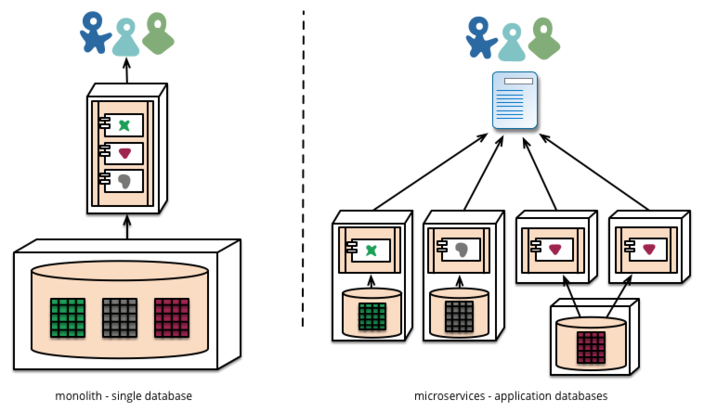
\includegraphics[width=0.8\textwidth]{microvsmono.png}
	\caption{Arquitecturas monolítica y microservicios.}\label{fig:microvsmono.png}
\end{figure}

Estos beneficios por supuesto vienen con desventajas:

\begin{enumerate}
\item Distribución: Raramente se van a ver microservicios en una arquitectura que no este distribuida, esto hace que sea más difícil de programar y tengamos que tener en cuenta otros errores.
\item Seguridad: Es más difícil asegurar la seguridad de un microservicio ya que debemos protegernos contra más puntos de vulnerabilidad, a no ser que estemos ejecutando en un clúster seguro.
\item Complejidad de operación: Hace falta un equipo de operaciones con madurez de manera que se puedan redistribuir los microsistemas regularmente.
\item Test a nivel de sistema: Los tests a nivel de sistema incrementan algo su complejidad ya que vamos a tener que usar microservicios falsos como mocks o similares casi siempre a no ser que estemos en un sistema pequeño.
\end{enumerate}

Por ultimo vale la pena hablar del coste en productividad, esto no es una ventaja ni un perjuicio, es un \textit{trade-off}, un intercambio.

En un sistema monolítico tenemos menos coste en productividad hasta que llegamos a un punto crítico en el que la complejidad aumenta demasiado o necesitamos escalar.

En los microservicios tenemos menos coste a la hora de seguir iterando aumentando la complejidad de un sistema pero a cambio tenemos mayor barrera de entrada hasta tener el primer prototipo funcional y los desarrolladores tienen que aprender cómo programar bajo esta arquitectura.
